\chapter{POMDPs.jl: A Framework for Sequential Decision Making under Uncertainty} \label{chap:pomdpsjl}

Since exact optimal solutions to POMDPs can rarely be attained, most research into solving realistic problems involves empirical comparison between solution techniques.
Sharing solver software between researchers can greatly improve speed and quality of this work.
This chapter describes the POMDPs.jl software package created by the Stanford Intelligent Systems Lab (SISL) to make state-of-the-art POMDP solution methods easily accessible to students, researchers, and engineers.
All of the research in \cref{chap:multilane,chap:pomcpow} was conducted using this framework.

\todo{Use cases?}

\section{Challenges for POMDP-solving software}

A successful POMDP software framework must have, at a minimum, the following attributes: speed, flexibility, and ease of use. Achieving all of these attributes simultaneously is a major challenge.

\subsection{Speed}

Since POMDPs are difficult to solve\todo{Make stronger statement about computational complexity}, any computational slowdown such as unnecessary memory allocation or runtime type inference significantly reduces the maximum problem size that the framework can handle.
For this reason, POMDP algorithms must be compiled to efficient processor instructions with low overhead.

\subsection{Flexibility}

The set of problems that can be represented as a POMDP is extremely large and there are many possible characteristics that such problems might have.
A good POMDP software framework should try to accommodate as much of this set as possible.
A few of the most important model characteristics to support are outlined below.

\subsubsection{Partial and full observability}

When studying a POMDP problem, it is almost always important to analyze the underlying fully-observable problem.
Thus, a good POMDP framework should have first-class support for MDPs in addition to POMDPs.

\subsubsection{Continuous and discrete problems}

Some POMDPs have a finite number of states, actions, and observations, i.e. $|\sspace| < \infty$, $|\aspace| < \infty$, and $|\ospace| < \infty$.
However, many real world problems, notably robotics problems, are naturally formulated in spaces with uncountably infinite cardinality, e.g. $\sspace = \reals$, $\aspace = \reals$, and $\ospace = \reals$, multi-dimensional vector spaces, e.g. $\sspace = \reals^6$, or hybrid continuous-discrete spaces.
This means that the framework must not be constrained to use integers for state representation, but should be capable of using a range of structures including floating point numbers and arrays.

\subsubsection{Explicit vs generative model representation}

Some POMDP and MDP solution techniques use the explicit probability distributions $\tdist$ and $\odist$ to solve problems.
Thus, a successful framework must include a way to explicitly specify $\tdist$ and $\odist$.
On the other hand, explicitly specifying $\tdist$ and $\odist$ for many realistic problems is exceedingly difficult and tedious, and specifying a generative model is the only practical way to encode the problem.
Thus, a successful framework must also include generative model support.

\subsubsection{Online and offline solvers}

While some POMDP solution techniques seek exact offline solutions to small problems, many larger problems can only be practically solved online.
Thus a good POMDP framework must have first class support for solving offline and efficiently executing a policy online or executing a planner that does significant computation online.

\subsubsection{Policy representation}

The policies that different solution techniques yield can take a variety of forms.
Exact solution techniques typically attempt to find alpha vectors that encode an optimal policy \cite{kaelbling1998planning,kurniawati2008sarsop}, whereas others use finite state machines \cite{bai2010mcvi}.
Newer methods may use neural networks \cite{karkus2017qmdp} or other structures to store policies, so a successful framework must provide a flexible way to represent all of these structures.

\subsection{Ease of Use}

In addition to being flexible and performant, the framework must be easy to use.
It is possible to make a framework that is performant and flexible but so complex that it will not be adopted or will cause much time to be wasted in understanding and implementation.
For the framework to be considered a success, it must be adopted by the community and serve as an enabler rather than a hindrance to research.

\section{Previous frameworks}

A number of frameworks exist for solving sequential decision problems.
However, most frameworks are written from a reinforcement learning perspective and hence only support either fully observable problems or problems where the state is fully observable, or environments that can generate observations but do not provide access to the Markov state structure of the problem.
Examples from this class are BURLAP~\cite{diuk2008object}, RLPy~\cite{geramifard2015rlpy}, and rllab~\cite{duan2016benchmarking}.
The most closely related frameworks to POMDPs.jl are APPL~\citep{appl}, AI-Toolbox~\citep{aitoolbox}, and ZMDP~\citep{zmdp} in that they explicitly represent the state and partial observability.
\todo{Check if BURLAP and ai toolbox actually do what I say}

APPL is the most widely used and up to date of these POMDP frameworks.
It is written efficiently in C++ and is excellent from a speed perspective.
However, it has several shortcomings in terms of flexibility and ease of use.
First, though all of the solvers in APPL support the POMDPX file format for discrete, explicit problem definitions, flexibility is limited because there is not a unified interface for defining generative models or continuous explicit models.
Second, prototyping problems and solvers in this framework is relatively time consuming and complex, making it difficult to use.
Specifically, the POMDPX file format is based on XML and is difficult for humans to write directly, so, in most cases, custom scripts must be written to create the files, and solvers and generative models written in C++ have higher development time costs than those written in a higher level language.

\todo{Check to make sure there is not a unified distribution}
\todo{Get quote from APPL}

Though much research progress has been made with these frameworks, POMDPs.jl offers several significant improvements.

\section{Architecture}

POMDPs.jl is designed to facilitate communication between different people performing three actions: defining problems, writing solver software, and running simulation experiments.
The same person will often operate in two or even all three of these roles, but will nearly always bring in some tools written by others.

The framework derives its solutions to the challenges outlined above primarily through the use of the Julia language itself \cite{bezanson2017julia}.
Julia is just-in-time compiled using the state-of-the art LLVM compiler framework, giving it speed comparable to traditional compiled languages such as C and C++.
However, unlike other compiled languages, it has many features that make numerical software development easier and faster.
For example, like Python, it is dynamically typed, has a powerful and flexible type system, and uses a modern, convenient syntax with features like list comprehensions, and, like Matlab, it has built-in efficient multidimensional arrays and linear algebra.
The makes meeting the flexibility and ease-of-use goals much easier.

\todo{cite LLVM}
\todo{Make sure Julia is dynamically typed}

This section describes some of the concepts used in the framework before outlining the interface itself.

\subsection{Concepts} \label{sec:concepts}

To fulfill each of the roles mentioned above, a programmer implements one or more classes that concretely represent concepts used to describe POMDP solving.
The problem writer creates a concrete subtype of the \texttt{POMDP} or \texttt{MDP} abstract classes to represent a problem, the simulator writer creates a \texttt{Simulator} type to run simulations, and the solver writer creates a \texttt{Solver} subtype to run computations offline, and a \texttt{Policy} subtype to execute a policy online.

In POMDPs.jl the term ``Belief'' is used to mean any structure that encodes the information needed to execute the policy.
For instance, if the policy is encoded as a set of alpha vectors, the belief takes its usual meaning as an explicit probability distribution over the states; for an online solver like POMCP, it must generate states for the tree search; and for a finite-state-machine policy like the one created by MCVI, it is simply the id of the current node.
An \texttt{Updater} in POMDPs.jl is an object that defines how information from new observations is integrated into the belief.
For example, if the belief is a probability distribution, the updater would apply Bayes rule or an approximation.
Since the belief is often closely related to the policy, the solver writer will often implement the \texttt{Updater}, however generic updaters such as particle filters are also available.
\Cref{fig:concepts} shows the three role concepts and some of the associated abstract types and interface functions.

\begin{figure}[htpb]
    \centering
    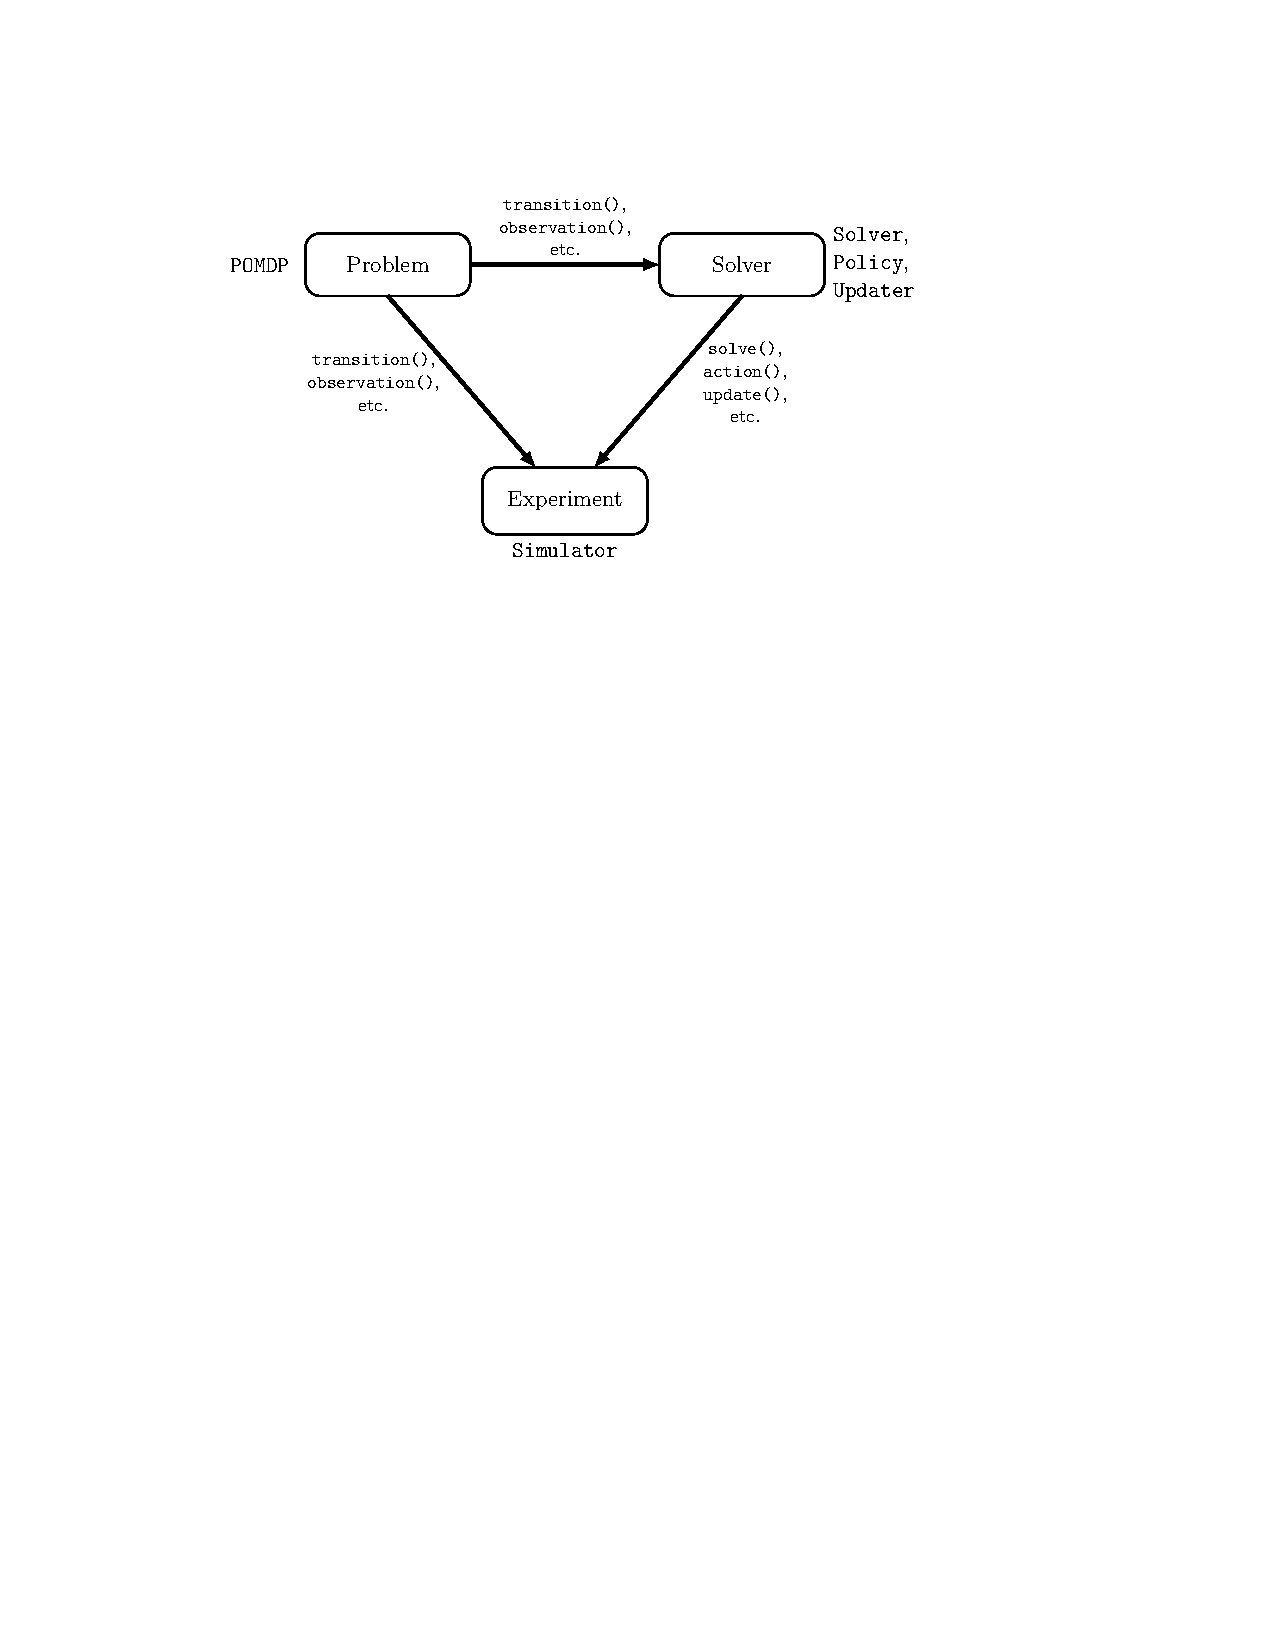
\includegraphics[width=0.8\linewidth]{media/arch.pdf}
    \caption[POMDPs.jl concepts]{POMDPs.jl concepts. POMDPs.jl facilitates communication between people in three roles. The abstract types are shown beside each node and some of the interface functions are shown between the nodes. The arrows indicate which roles use code from which other roles.}
    \label{fig:concepts}
\end{figure}

\subsection{Interfaces}

The behavior of POMDPs.jl objects is defined by implementing methods of interface functions.
Implementing interface functions serves as an alternative to writing configuration files such as POMDPX files or specifications in purpose-built languages like RDDL~\cite{sanner2010rddl} in previous frameworks.
For example the problem writer may implement a method of the \texttt{reward} function that returns the reward given a problem instance, state and action.
Julia will call the correct \texttt{reward} method for the problem type based on its multiple dispatch system \cite{bezanson2017julia}.
Similarly, an \texttt{Updater} should have a corresponding \texttt{update} method that returns a new belief given an updater object, previous belief, action, and observation.
The complete interface is not listed here, but is available in the online documentation.

In POMDPs.jl, states, actions, observations, beliefs, and distributions can be represented by objects of any type as long as the appropriate interface methods are implemented.
This provides the flexibility needed to represent continuous or discrete problems.
Packages in the Julia ecosystem provide convenient and efficient types for common state representations, such as small fixed-size vectors.

One flexibility goal that has not been met by previous frameworks is support of both generative and explicit problem definitions.
For example, in APPL, all solvers can handle POMDPX problem specification for explicit definitions, but the MCVI and DESPOT solvers use different interfaces for generative problems, and there is no way to represent continuous problems explicitly.
POMDPs.jl overcomes this challenge by exposing both an explicit interface and generative interface that can be mixed.
If the necessary parts of the explicit interface are implemented for a problem, POMDPs.jl will automatically provide the generative interface functions for the problem.
The interface relationships are illustrated in \cref{fig:interfaces}.
Implementations of all of the interface functions are not strictly required; if the minimum set of functions used by a solver or simulator are implemented for a problem, then that solver or simulator will work with that problem.

\begin{figure}[htpb]
    \centering
    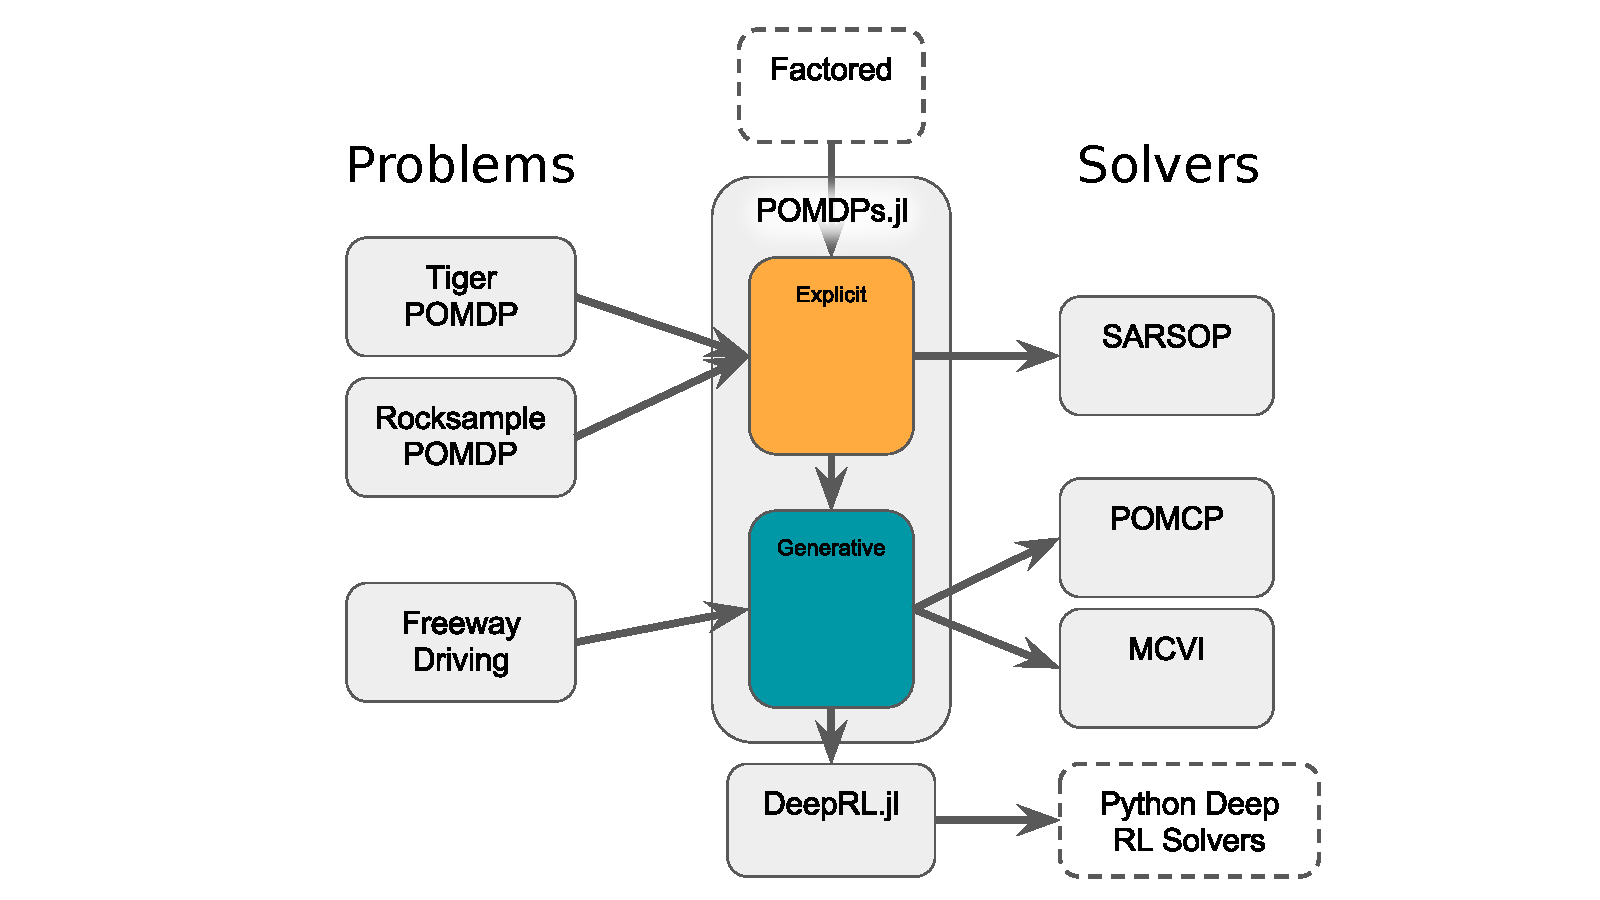
\includegraphics[width=0.8\linewidth]{media/interfaces.pdf}
    \caption{POMDPs.jl interfaces}
    \label{fig:interfaces}
\end{figure}

Because of the interface's flexibility, expressing which interface functions a problem-writer should implement, giving helpful error messages, and even checking whether a sufficient portion of the interface has been implemented is a complex challenge.
For example, suppose a user intends to implement a complex problem that cannot easily be expressed with an explicit definition and intends to use a solver that only requires functions from the generative interface.
If POMDPs.jl advises this user to implement functions from the explicit interface, he or she will conclude that expressing the problem is difficult or impossible.
This complexity drove the development of an interface and framework for dynamically specifying requirements and dependencies and generating helpful reports for users.
In this requirements framework, built with Julia's powerful metaprogramming features, solver and simulator writers declare the requirements for their algorithm, which may be based on solver options, and problem writers can check which of the requirements have been satisfied by their problem implementation.
Examples of the output of this system are shown in \cref{fig:requirements}.

\begin{figure}[htpb]
    \centering
    \begin{subfigure}[b]{0.48\textwidth}
    \begin{center}
        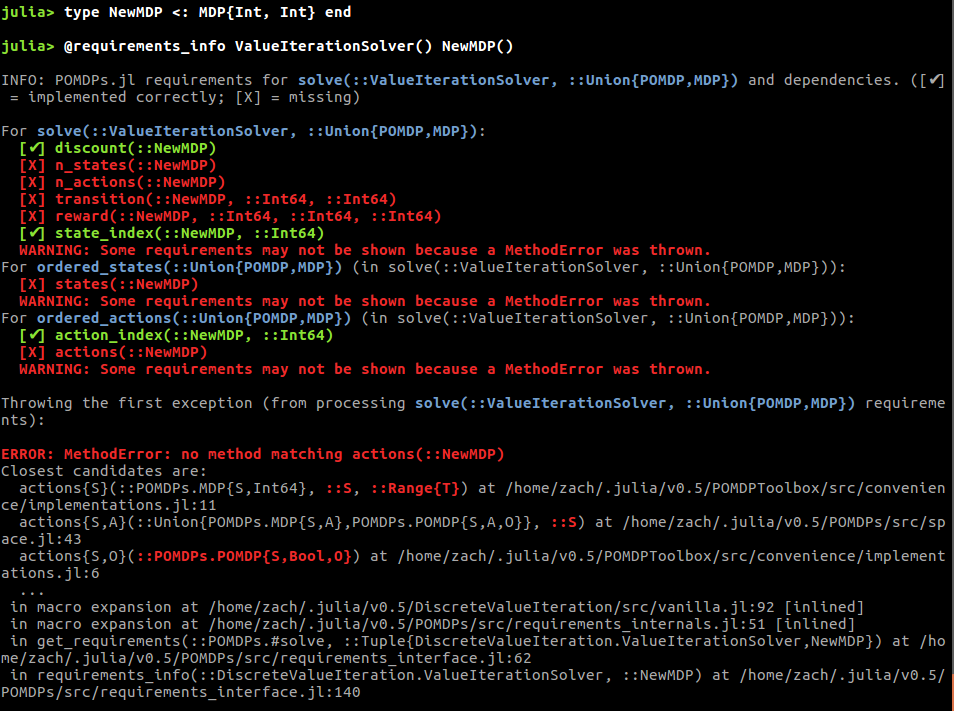
\includegraphics[width=\textwidth]{media/requirements_info_new.png}
    \end{center}
    \caption{New problem with no methods}
    \end{subfigure}
    \hfill
    \begin{subfigure}[b]{0.48\textwidth}
    \begin{center}
        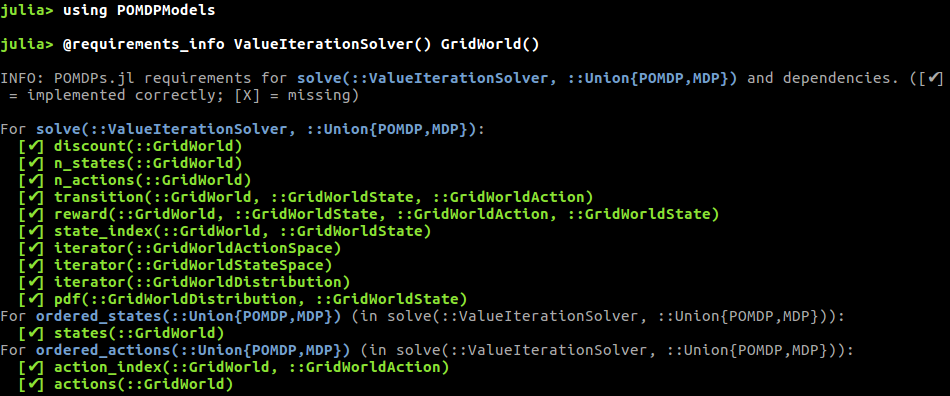
\includegraphics[width=\textwidth]{media/requirements_info_gw.png}
    \end{center}
    \caption{Fully implemented problem}
    \end{subfigure}
     
    \caption[POMDPs.jl requirements example]{POMDPs.jl requirements example output for the value iteration solver}
    \label{fig:requirements}
\end{figure}

\section{Example}

This section presents simple examples illustrating implementations of the concepts in~\cref{sec:}, namely the problem, the solver, and the experiment. 
The POMDPs.jl interface consists of several abstract types and a set of functions that support these concepts. 

% \lstset{escapechar=@,style=customjulia}
% 
% %\begin{lstlisting}
%  %using POMDPs       # loads the interface
%  %POMDPs.add("QMDP") # installs a supported JuliaPOMDP package and its deps
% %\end{lstlisting}
% 
% 
% \noindent \textbf{Problem:} 
% The problem defines the MDP or POMDP model to be solved.
% %The user decides how to define the model components.
% Below is a definition for the Tiger POMDP~\citep{kaelbling1998planning}.
% 
% % \begin{lstlisting}
% %  type TigerState s::Bool end
% %  type TigerPOMDP <: POMDP{TigerState, Int64, Bool}
% %      p_correct::Float64     # probability of hearing the tiger correctly
% %      discount::Float64      # discount factor
% %  end
% % \end{lstlisting}
% \begin{lstlisting}
%  immutable TigerPOMDP <: POMDP{Bool, Int64, Bool}
%      p_correct::Float64     # probability of hearing the tiger correctly
%      discount::Float64      # discount factor
%  end
% \end{lstlisting}
% 
% \noindent The {\small\ttfamily TigerPOMDP} type inherits from the abstract {\small\ttfamily POMDP} type (part of the POMDPs.jl interface), which is parametrized by the state, action, and observation types. 
% % The state can be represented with a custom {\small\ttfamily TigerState} type or with a native {\small\ttfamily Bool} type.
% In this case, the state is represented by the native {\small\ttfamily Bool} type, but, in general, these types may be user-defined.
% The same flexibility is available for the other components of the problem, giving the user the flexibility to define their problem in the form of their choosing. 
% 
% \iffalse
% \begin{lstlisting}
%  type TigerPOMDP <: POMDP{Bool, Int64, Bool}
%      r_listen::Float64      # reward for listening (negative)
%      r_findtiger::Float64   # reward for finding tiger (negative)
%      r_escapetiger::Float64 # reward for escaping the tiger
%      p_correct::Float64     # probability of hearing the tiger correctly
%      discount::Float64      # discount factor
%  end
% \end{lstlisting}
% \fi
% 
% 
% % removed figure
% \iffalse
% \begin{figure}
% \begin{lstlisting}[basicstyle=\small\ttfamily]
%     type BabyPOMDP <: POMDP{Bool, Bool, Bool}
%         r_feed::Float64                # reward for feeding (negative)
%         r_hungry::Float64              # reward for being hungry (negative)
%         p_become_hungry::Float64       # probability of becoming hungry
%         p_cry_when_hungry::Float64     # probability of crying when hungry
%         p_cry_when_not_hungry::Float64 # probability of crying when not hungry
%         discount::Float64              # discount factor
%     end
%     ...
%     type BoolDistribution <: AbstractDistribution{Bool}
%         p::Float64                     # probability of true
%     end
%     ...
%     function transition(pomdp::BabyPOMDP, s::Bool, a::Bool, d::BoolDistribution)
%         if !a && s                     # did not feed when hungry
%             d.p = 1.0
%         elseif a                       # fed
%             d.p = 0.0
%         else                           # did not feed when not hungry
%             d.p = pomdp.p_become_hungry
%         end
%         return d
%     end
%     ...
% \end{lstlisting}
% \caption{Sample code from the implementation of a POMDP problem. The elipses indicate locations where code has been omitted.}
% \label{fig:problem}
% \end{figure}
% \fi
% 
% 
% \noindent \textbf{Solver:} 
% A solver implementation typically requires three type definitions: a {\small\ttfamily Solver} that contains the parameters that define solver behavior, a {\small\ttfamily Policy} that defines a mapping from beliefs to actions, and an {\small\ttfamily Updater} that defines how the belief is updated with new observations.
% An example of a QMDP~\citep{littman1995} policy type is shown below.
% %\todo[author=EB, inline]{So, we are ok defining belief updater as part of the solver?}
% 
% \begin{lstlisting}
%  type QMDPPolicy{Action} <: Policy
%      alphas::Matrix{Float64}    # policy alpha vectors
%      action_map::Vector{Action} # indices to actions  
%      pomdp::POMDP    	       # POMDP model
%  end
% \end{lstlisting}
% 
% \noindent A solver implementation usually includes three top-level functions: {\small\ttfamily solve}, that creates a policy for the problem given the solver, {\small\texttt{action}}, that emits an action for a belief based on the policy, and {\small\texttt{update}}, that updates the belief based on the action taken and the observation received, given the updater.
% 
% 
% \noindent \textbf{Experiment:} 
% Experiments combine problems and solvers to evaluate the quality of a solver policy.
% For example, the experimenter might create a simulator type, {\ttfamily Sim}, and a corresponding {\ttfamily simulate} function (an important part of the main loop is shown below).
% \begin{lstlisting}
%  function simulate(sim::Sim, pomdp, policy, updater, initial_dist)
%     ...
%     for t in 1:sim.max_steps
%         a = action(policy, b)
%         sp = rand(sim.rng, transition(pomdp, s, a))
%         r_total += discount(pomdp)^t*reward(pomdp, s, a, sp)
%         o = rand(sim.rng, observation(pomdp, s, a, sp))
%         b = update(updater, b, a, o)
%         ...
% \end{lstlisting}
% A simulation can then be run as follows: 
% \begin{lstlisting}
%  using QMDP, POMDPModels, POMDPToolbox # import JuliaPOMDP packages
%  pomdp = TigerPOMDP()                  # initialize the tiger problem
%  solver = QMDPSolver()                 # initialize QMDP solver
%  policy = solve(solver, pomdp)         # compute a policy
%  r = simulate(Sim(), pomdp, policy, updater(policy), DiscreteBelief(2))
% \end{lstlisting}





